% Options for packages loaded elsewhere
\PassOptionsToPackage{unicode}{hyperref}
\PassOptionsToPackage{hyphens}{url}
%
\documentclass[
]{article}
\usepackage{lmodern}
\usepackage{amssymb,amsmath}
\usepackage{ifxetex,ifluatex}
\ifnum 0\ifxetex 1\fi\ifluatex 1\fi=0 % if pdftex
  \usepackage[T1]{fontenc}
  \usepackage[utf8]{inputenc}
  \usepackage{textcomp} % provide euro and other symbols
\else % if luatex or xetex
  \usepackage{unicode-math}
  \defaultfontfeatures{Scale=MatchLowercase}
  \defaultfontfeatures[\rmfamily]{Ligatures=TeX,Scale=1}
\fi
% Use upquote if available, for straight quotes in verbatim environments
\IfFileExists{upquote.sty}{\usepackage{upquote}}{}
\IfFileExists{microtype.sty}{% use microtype if available
  \usepackage[]{microtype}
  \UseMicrotypeSet[protrusion]{basicmath} % disable protrusion for tt fonts
}{}
\makeatletter
\@ifundefined{KOMAClassName}{% if non-KOMA class
  \IfFileExists{parskip.sty}{%
    \usepackage{parskip}
  }{% else
    \setlength{\parindent}{0pt}
    \setlength{\parskip}{6pt plus 2pt minus 1pt}}
}{% if KOMA class
  \KOMAoptions{parskip=half}}
\makeatother
\usepackage{xcolor}
\IfFileExists{xurl.sty}{\usepackage{xurl}}{} % add URL line breaks if available
\IfFileExists{bookmark.sty}{\usepackage{bookmark}}{\usepackage{hyperref}}
\hypersetup{
  pdftitle={Presentación dispocen},
  hidelinks,
  pdfcreator={LaTeX via pandoc}}
\urlstyle{same} % disable monospaced font for URLs
\usepackage[margin=1in]{geometry}
\usepackage{color}
\usepackage{fancyvrb}
\newcommand{\VerbBar}{|}
\newcommand{\VERB}{\Verb[commandchars=\\\{\}]}
\DefineVerbatimEnvironment{Highlighting}{Verbatim}{commandchars=\\\{\}}
% Add ',fontsize=\small' for more characters per line
\usepackage{framed}
\definecolor{shadecolor}{RGB}{248,248,248}
\newenvironment{Shaded}{\begin{snugshade}}{\end{snugshade}}
\newcommand{\AlertTok}[1]{\textcolor[rgb]{0.94,0.16,0.16}{#1}}
\newcommand{\AnnotationTok}[1]{\textcolor[rgb]{0.56,0.35,0.01}{\textbf{\textit{#1}}}}
\newcommand{\AttributeTok}[1]{\textcolor[rgb]{0.77,0.63,0.00}{#1}}
\newcommand{\BaseNTok}[1]{\textcolor[rgb]{0.00,0.00,0.81}{#1}}
\newcommand{\BuiltInTok}[1]{#1}
\newcommand{\CharTok}[1]{\textcolor[rgb]{0.31,0.60,0.02}{#1}}
\newcommand{\CommentTok}[1]{\textcolor[rgb]{0.56,0.35,0.01}{\textit{#1}}}
\newcommand{\CommentVarTok}[1]{\textcolor[rgb]{0.56,0.35,0.01}{\textbf{\textit{#1}}}}
\newcommand{\ConstantTok}[1]{\textcolor[rgb]{0.00,0.00,0.00}{#1}}
\newcommand{\ControlFlowTok}[1]{\textcolor[rgb]{0.13,0.29,0.53}{\textbf{#1}}}
\newcommand{\DataTypeTok}[1]{\textcolor[rgb]{0.13,0.29,0.53}{#1}}
\newcommand{\DecValTok}[1]{\textcolor[rgb]{0.00,0.00,0.81}{#1}}
\newcommand{\DocumentationTok}[1]{\textcolor[rgb]{0.56,0.35,0.01}{\textbf{\textit{#1}}}}
\newcommand{\ErrorTok}[1]{\textcolor[rgb]{0.64,0.00,0.00}{\textbf{#1}}}
\newcommand{\ExtensionTok}[1]{#1}
\newcommand{\FloatTok}[1]{\textcolor[rgb]{0.00,0.00,0.81}{#1}}
\newcommand{\FunctionTok}[1]{\textcolor[rgb]{0.00,0.00,0.00}{#1}}
\newcommand{\ImportTok}[1]{#1}
\newcommand{\InformationTok}[1]{\textcolor[rgb]{0.56,0.35,0.01}{\textbf{\textit{#1}}}}
\newcommand{\KeywordTok}[1]{\textcolor[rgb]{0.13,0.29,0.53}{\textbf{#1}}}
\newcommand{\NormalTok}[1]{#1}
\newcommand{\OperatorTok}[1]{\textcolor[rgb]{0.81,0.36,0.00}{\textbf{#1}}}
\newcommand{\OtherTok}[1]{\textcolor[rgb]{0.56,0.35,0.01}{#1}}
\newcommand{\PreprocessorTok}[1]{\textcolor[rgb]{0.56,0.35,0.01}{\textit{#1}}}
\newcommand{\RegionMarkerTok}[1]{#1}
\newcommand{\SpecialCharTok}[1]{\textcolor[rgb]{0.00,0.00,0.00}{#1}}
\newcommand{\SpecialStringTok}[1]{\textcolor[rgb]{0.31,0.60,0.02}{#1}}
\newcommand{\StringTok}[1]{\textcolor[rgb]{0.31,0.60,0.02}{#1}}
\newcommand{\VariableTok}[1]{\textcolor[rgb]{0.00,0.00,0.00}{#1}}
\newcommand{\VerbatimStringTok}[1]{\textcolor[rgb]{0.31,0.60,0.02}{#1}}
\newcommand{\WarningTok}[1]{\textcolor[rgb]{0.56,0.35,0.01}{\textbf{\textit{#1}}}}
\usepackage{graphicx,grffile}
\makeatletter
\def\maxwidth{\ifdim\Gin@nat@width>\linewidth\linewidth\else\Gin@nat@width\fi}
\def\maxheight{\ifdim\Gin@nat@height>\textheight\textheight\else\Gin@nat@height\fi}
\makeatother
% Scale images if necessary, so that they will not overflow the page
% margins by default, and it is still possible to overwrite the defaults
% using explicit options in \includegraphics[width, height, ...]{}
\setkeys{Gin}{width=\maxwidth,height=\maxheight,keepaspectratio}
% Set default figure placement to htbp
\makeatletter
\def\fps@figure{htbp}
\makeatother
\setlength{\emergencystretch}{3em} % prevent overfull lines
\providecommand{\tightlist}{%
  \setlength{\itemsep}{0pt}\setlength{\parskip}{0pt}}
\setcounter{secnumdepth}{-\maxdimen} % remove section numbering
\usepackage{booktabs}
\usepackage{longtable}
\usepackage{array}
\usepackage{multirow}
\usepackage{wrapfig}
\usepackage{float}
\usepackage{colortbl}
\usepackage{pdflscape}
\usepackage{tabu}
\usepackage{threeparttable}
\usepackage{threeparttablex}
\usepackage[normalem]{ulem}
\usepackage{makecell}
\usepackage{xcolor}

\title{Presentación dispocen}
\author{}
\date{\vspace{-2.5em}}

\begin{document}
\maketitle

En este documento se presenta una librería de herramientas en lo que
pretende ser una guía rápida de uso para el cálculo de la disponibilidad
léxica, la centralidad léxica y las diferentes funcionalidades que de
esta última se derivan. Aunque la librería permite, a través de
programación funcional, implementar múltiples modelos, se proporciona un
conjunto de herramientas elementales prediseñadas para que se pueda
empezar a usar con las funciones señaladas (disponibilidad, centralidad)
de forma casi inmediata. Sin embargo, consideramos necesario hacer notar
que estas posibilidades de aplicación directa representan tan solo un
subconjunto de las opciones que permite el sistema aquí presentado.

Actualmente está en preparación otro trabajo en el que se discuten en
profundidad tanto los modelos posibles y las diferentes opciones de
aplicación, como un estudio de diferentes aspectos de las bases teóricas
del cálculo de la disponibilidad y su interpretación. Sin embargo, el
desarrollo de estas etapas posteriores requiere cierta destreza en el
manejo de la sintaxis de R y de conceptos de programación funcional, con
lo que su presentación requiere otro ámbito de exposición.

\hypertarget{exposiciuxf3n-y-contextualizaciuxf3n-del-sistema}{%
\section{Exposición y contextualización del
sistema}\label{exposiciuxf3n-y-contextualizaciuxf3n-del-sistema}}

El sistema se ha construido sobre R\footnote{\url{https://www.r-project.org/}},
una implementación abierta del lenguaje de programación S, que lleva en
desarrollo desde 1992 y con una primera versión estable en el año 2000.
Es fácilmente extensible y permite la reutilización de código y datos.
Se trata de un sistema soportado por una amplia comunidad a lo largo del
mundo y se usa de forma habitual en entornos de análisis de datos de
ingeniería y medicina.

RStudio\footnote{\url{https://rstudio.com/}} es un entorno comercial de
desarrollo para R que permite el uso personal gratuito y que aumenta la
productividad en el uso de este lenguaje. Está disponible para la gran
mayoría de plataformas y sistemas operativos. Para facilitar el trabajo,
se proporcionan utilidades que se pueden ejecutar dentro de este entorno
y que facilitan el proceso de análisis.

Es posible utilizar las funcionalidades proporcionadas por nuestro
software sin el uso de RStudio, pero consideramos que su empleo se
dificulta y se pierden muchas de las posibilidades que proporciona este
marco de software.

Dentro del sistema construido en RStudio nos resulta especialmente
interesante la posibilidad de usar el paradigma de la \emph{programación
literaria}, según la cual, en un mismo documento, se integran tanto los
contenidos textuales como la exposición de hechos o la interpretación de
los análisis a través de bloques de código que llevan a cabo las
manipulaciones y representaciones de datos. Lo que sigue pretende ser un
ejemplo práctico del uso de esta metodología. Como muestra de sus
ventajas --al incluir en el mismo documento el análisis que se ha
llevado a cabo con el código para realizarlo-- se potencia la
replicabilidad, característica cada vez más exigida en el mundo
académico, en la que se debe permitir que otros investigadores puedan
replicar, tanto para verificar como para desarrollar de manera
individual, el trabajo expuesto. Este objetivo se cumple al exponer en
el mismo documento la disertación y el código con el que se ha realizado
los análisis.

A diferencia de soluciones basadas en programas autónomos para el
cálculo de la disponibilidad léxica, la implementación de esta solución
dentro de un sistema como el formado por R junto con RStudio permite,
además, la integración de todo el procedimiento de gestión de datos. De
esta forma, los resultados obtenidos a partir de las herramientas
proporcionadas se incorporan al sistema, con lo que se permite la
integración en nuevos procesos de datos y la aplicación personal de los
resultados obtenidos.

La distribución de las soluciones es otro problema que ya ha encontrado
soluciones eficientes dentro de la comunidad de usuarios de \texttt{R}.
Repositorios de código como GitHub permiten la gestión y el control
automatizado de versiones. Es posible llevar a cabo un control
exhaustivo de las modificaciones que se van realizando, sin necesidad de
descargar e instalar continuamente programas. Con dos líneas de código
podemos estar seguros de tener instalada la última versión disponible.
Además, este modelo de intercambio de código permite que los proyectos
no desaparezcan, ya que se pueden crear ramas de cualquier repositorio
de código para continuar su desarrollo, independientemente de los
creadores originales.

Entre las múltiples herramientas construidas sobre \texttt{R} hemos
considerado muy interesantes y productivas las herramientas que
conforman el ``Universo Tidyverse''\footnote{\url{https://www.tidyverse.org/}}.
Se trata de un conjunto de librerías que facilitan y permiten una
manipulación expresiva de los datos, basada en el concepto de tubería.
Este tratamiento se construye mediante la secuenciación de
manipulaciones que se van encadenando, de manera que el resultado de una
etapa se convierte en la fuente de datos para la siguiente. Esta
característica, junto con operadores adaptados a este tipo de trabajo,
proporciona una expresividad potente y cómoda de llevar a cabo
transformaciones que, de otra forma, serían muy complejas. Las
manipulaciones de datos presentadas en este trabajo se realizan
utilizando estas herramientas.

\hypertarget{instalaciuxf3n}{%
\section{Instalación}\label{instalaciuxf3n}}

\hypertarget{prerequisitos}{%
\subsection{Prerequisitos}\label{prerequisitos}}

En primer lugar es necesario instalar el sistema \texttt{R}. Para ello
se accede, en la sección \emph{Download} de la página del proyecto,
\url{https://www.r-project.org/}, al enlace
\href{http://cran.r-project.org/mirrors.html}{CRAN}, seleccionar un
sitio --en nuestro caso vamos a escoger el de la Red Iris, que es una
réplica local en España \url{https://cran.rediris.es/}-- y, en la página
principal encontramos un enlace para descargar la versión para nuestro
sistema operativo. En el caso de elegir la versión para Windows, se
elegiría la versión \texttt{base} y accedemos, finalmente, al binario
que instala el sistema, que en este momento, corresponde a la versión
\texttt{4.0.2}, en el enlace
(\url{https://cran.rediris.es/bin/windows/base/R-4.0.2-win.exe}){[}\url{https://cran.rediris.es/bin/windows/base/R-4.0.2-win.exe}{]}.

A continuación se recomienda, aunque no es estrictamente necesario,
instalar el entorno de productividad \texttt{RStudio}. En
(\url{https://rstudio.com/}){[}\url{https://rstudio.com/}{]}, siguiendo,
en este momento, el camino \texttt{Product} \textgreater{}
\texttt{Open\ Source} \textgreater{} \texttt{RStudio}, se llega a la
página de descripción del producto, del que hay dos versiones:
\texttt{Desktop} y \texttt{Server}. En nuestro caso usaremos la versión
\texttt{Desktop}, en su versión \emph{Open Source Edition}, que se puede
descargar en
(\url{https://rstudio.com/products/rstudio/download/}){[}\url{https://rstudio.com/products/rstudio/download/}{]}.
La versión actual para Windows se encuentra en
(\url{https://download1.rstudio.org/desktop/windows/RStudio-1.3.1073.exe}){[}\url{https://download1.rstudio.org/desktop/windows/RStudio-1.3.1073.exe}{]}.

\hypertarget{dispocen}{%
\subsection{dispocen}\label{dispocen}}

Una vez instalados los prerequisitos, para poder utilizar las
herramientas que proponemos, el usuario debe llevar a cabo un segundo
paso de instalación que, en nuestra opinión, no es más complejo que
cualquier proceso de instalación en el sistema \emph{R}. Este paso ha de
hacerse únicamente cuando se pretenda instalar o actualizar el paquete
en el sistema. Puesto que nuestra intención es seguir trabajando en el
paquete, sería recomendable realizar esta acción de forma periódica.

Las siguientes órdenes instalan el paquete \emph{dispocen} desde el
repositorio \emph{GitHub}. Todo el código está implementado en \emph{R},
con lo que es fácil de revisar.

\begin{Shaded}
\begin{Highlighting}[]
\KeywordTok{install.packages}\NormalTok{(}\StringTok{"devtools"}\NormalTok{)}
\KeywordTok{library}\NormalTok{(devtools)}
\KeywordTok{install_github}\NormalTok{(}\StringTok{"jmss70/dispocen"}\NormalTok{)}
\end{Highlighting}
\end{Shaded}

Para facilitar la introducción de la herramienta se han impuesto como
requerimientos, para que se instalen de forma automática, las
herramientas del universo \emph{Tidyverse}, que facilitan el
procesamiento de datos y se usa de forma extensiva en este y otros
trabajos, y la librería \emph{flextable} y \emph{kableExtra}, con el
objetivo de mejorar la presentación de las tablas.

Una vez que se han llevado a cabo los pasos anteriores, y si no se ha
producido ningún contratiempo, el sistema está preparado para ejecutar
el cálculo de los índices de disponibilidad y centralidad.

\hypertarget{carga-de-las-libreruxedas-y-los-datos}{%
\section{Carga de las librerías y los
datos}\label{carga-de-las-libreruxedas-y-los-datos}}

Para poder usar las librerías hay que cargarlas en nuestra sesión de
trabajo. De esta manera se ponen a disposición del usuario las funciones
que proporcionan.

\begin{Shaded}
\begin{Highlighting}[]
\KeywordTok{library}\NormalTok{(dispocen)}
\end{Highlighting}
\end{Shaded}

El formato requerido de los datos coincide con el tradicionalmente usado
por los programas más empleados hasta ahora para el cálculo de la
disponibilidad léxica (\textbf{Lexidisp}, \textbf{Dispolex},
esencialmente). Sin embargo, consideramos que parte de la información
que contiene su estructura es redundante y sería conveniente plantear la
posibilidad de establecer un estándar de codificación que sea más
coherente con los modelos de datos normalizados.

De momento, se espera que los datos estén en un archivo de texto, con
campos separados por espacios, según el siguiente formato:

\begin{itemize}
\tightlist
\item
  Un campo con información sociológica básica del hablante formada por
  cinco caracteres sucesivos. Cada uno de ellos representa la
  codificación de una variante dentro de una variable sociológica
\item
  Un campo de identificación del usuario de tres caracteres
\item
  Un campo de identificación del centro de interés de dos caracteres
\item
  Una lista de palabras separadas por comas y siguiendo el orden de su
  aparición en las listas originales. Es necesario que no se utilice el
  carácter ``coma'' como valor de un elemento, ya que se interpretaría
  como separador.
\end{itemize}

Un ejemplo de dos líneas sería:

\begin{verbatim}
21131 001 01 mano, pie, brazo, cerebro, pulmón, nariz, extremidad, ojo, boca, diente, pelo, oreja, culo, vagina 
12131 002 01 riñón, corazón, garganta, cabeza, pierna, pie, hígado, estómago, mano, brazo, antebrazo, abdomen, pecho, ojo, boca, oído, dedo, rodilla, costilla 
\end{verbatim}

Suponiendo que tenemos todos los datos cargados en un archivo,
denominado \texttt{datos.txt}, que estará alojado en el mismo directorio
que el script de procesamiento, se podrían cargar los datos como:

\begin{Shaded}
\begin{Highlighting}[]
\NormalTok{data <-}\StringTok{ }\KeywordTok{read.dispocen}\NormalTok{(}\StringTok{"datos.txt"}\NormalTok{)}
\NormalTok{data }\OperatorTok\StringTok{ }
\StringTok{  }\KeywordTok{head}\NormalTok{() }\OperatorTok\StringTok{ }
\StringTok{  }\KeywordTok{flextable}\NormalTok{() }\OperatorTok\StringTok{ }\KeywordTok{autofit}\NormalTok{() }\OperatorTok
\StringTok{  }\KeywordTok{theme_booktabs}\NormalTok{()}
\end{Highlighting}
\end{Shaded}

\begin{verbatim}
## PhantomJS not found. You can install it with webshot::install_phantomjs(). If it is installed, please make sure the phantomjs executable can be found via the PATH variable.
\end{verbatim}

\includegraphics[width=3.20in,height=2.16in,keepaspectratio]{PresentacionCentralex_files/figure-latex/unnamed-chunk-3-1.png}

\hypertarget{cuxe1lculo-de-la-disponibilidad}{%
\section{Cálculo de la
disponibilidad}\label{cuxe1lculo-de-la-disponibilidad}}

La función general del cálculo de la disponibilidad es
\texttt{build.availability}. Sin embargo, el uso de esta función
requiere del uso de varios parámetros. Se han construidos dos funciones
de utilidad que encapsulan su uso y ofrecen los dos modelos que
consideramos, por el momento, más interesantes (Modelo
López-Strassburger y Modelo Ávila-Sánchez). Consideramos que es
preferible exponer su uso mediante ejemplos.

\hypertarget{modelo-de-luxf3pez-strassburger}{%
\subsection{Modelo de
López-Strassburger}\label{modelo-de-luxf3pez-strassburger}}

Este modelo, que es el más conocido y el último de una serie de
iteraciones para la cuantificación de la disponibilidad, se puede usar
como:

\begin{Shaded}
\begin{Highlighting}[]
\NormalTok{disponibilidad <-}\StringTok{ }\KeywordTok{build.lopezstrass.availability}\NormalTok{(data)}
\end{Highlighting}
\end{Shaded}

El resultado es un nuevo marco de datos cuyos campos son el centro de
interés, la palabra y la disponibilidad calculada, junto con otros datos
necesarios para su obtención como la posición y las frecuencias
relativas y acumuladas dentro del centro de interés:

\begin{Shaded}
\begin{Highlighting}[]
\KeywordTok{head}\NormalTok{(disponibilidad) }\OperatorTok
\StringTok{  }\KeywordTok{flextable}\NormalTok{() }\OperatorTok\StringTok{ }
\StringTok{  }\KeywordTok{set_header_labels}\NormalTok{(}\DataTypeTok{centers =} \StringTok{"Centro de interés"}\NormalTok{, }
                    \DataTypeTok{words=}\StringTok{"Palabra"}\NormalTok{, }
                    \DataTypeTok{order=}\StringTok{"Orden"}\NormalTok{, }
                    \DataTypeTok{availability=}\StringTok{"Disponibilidad"}\NormalTok{, }
                    \DataTypeTok{freq.abs=}\StringTok{"Frecuencia absoluta"}\NormalTok{, }
                    \DataTypeTok{freq.abs.cum=}\StringTok{"Frecuencia absoluta acumulada"}\NormalTok{, }
                    \DataTypeTok{freq.rel=}\StringTok{"Frecuencia relativa"}\NormalTok{, }
                    \DataTypeTok{freq.rel.cum=}\StringTok{"Frecuencia relativa acumulada"}\NormalTok{) }\OperatorTok
\StringTok{  }\KeywordTok{colformat_num}\NormalTok{(}\DataTypeTok{j=}\KeywordTok{c}\NormalTok{(}\DecValTok{4}\NormalTok{,}\DecValTok{6}\NormalTok{,}\DecValTok{8}\NormalTok{), }\DataTypeTok{digits=}\DecValTok{6}\NormalTok{) }\OperatorTok
\StringTok{  }\KeywordTok{width}\NormalTok{(}\DataTypeTok{j=}\KeywordTok{c}\NormalTok{(}\DecValTok{1}\NormalTok{,}\DecValTok{3}\NormalTok{,}\DecValTok{5}\NormalTok{,}\DecValTok{7}\NormalTok{),}\DataTypeTok{width=}\NormalTok{.}\DecValTok{65}\NormalTok{) }\OperatorTok
\StringTok{  }\KeywordTok{width}\NormalTok{(}\DataTypeTok{j=}\KeywordTok{c}\NormalTok{(}\DecValTok{2}\NormalTok{,}\DecValTok{4}\NormalTok{,}\DecValTok{6}\NormalTok{,}\DecValTok{8}\NormalTok{),}\DataTypeTok{width=}\NormalTok{.}\DecValTok{9}\NormalTok{) }\OperatorTok
\StringTok{  }\KeywordTok{theme_booktabs}\NormalTok{()}
\end{Highlighting}
\end{Shaded}

\begin{verbatim}
## PhantomJS not found. You can install it with webshot::install_phantomjs(). If it is installed, please make sure the phantomjs executable can be found via the PATH variable.
\end{verbatim}

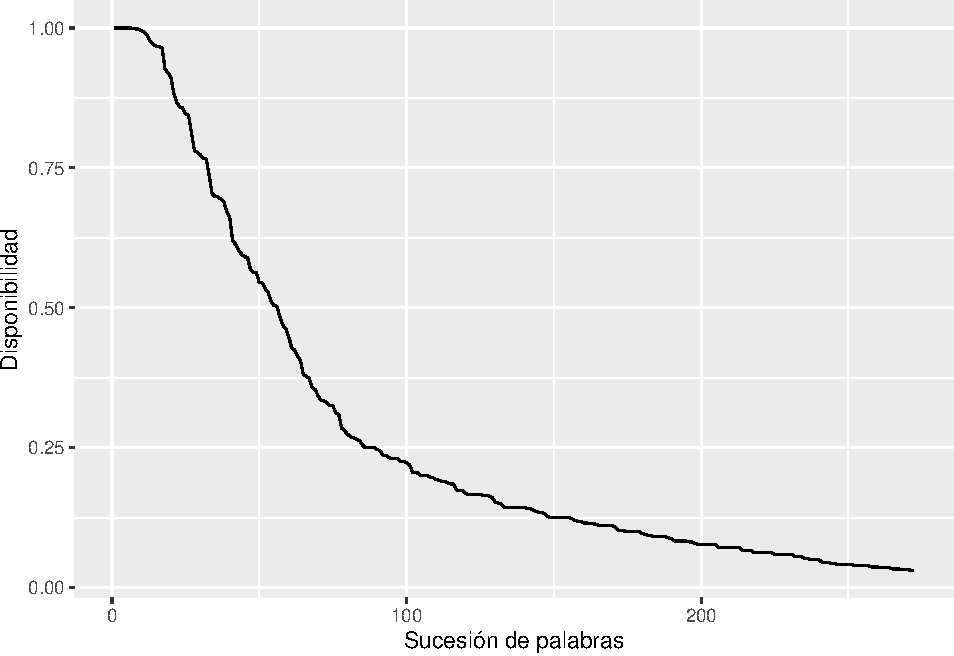
\includegraphics[width=6.20in,height=1.75in,keepaspectratio]{PresentacionCentralex_files/figure-latex/unnamed-chunk-5-1.png}
Al ser un marco de datos de \emph{R} estándar, se pueden realizar sobre
él todas las operaciones que permite el sistema. En el siguiente ejemplo
hemos seleccionado los resultados obtenidos en el centro de interés
``03'', los hemos ordenado en orden decreciente de disponibilidad y
mostramos los 10 vocablos más disponibles

\begin{Shaded}
\begin{Highlighting}[]
\NormalTok{disponibilidad }\OperatorTok\StringTok{ }
\StringTok{  }\KeywordTok{filter}\NormalTok{(centers}\OperatorTok{==}\StringTok{"03"}\NormalTok{) }\OperatorTok\StringTok{ }
\StringTok{  }\KeywordTok{arrange}\NormalTok{(}\OperatorTok{-}\NormalTok{availability) }\OperatorTok\StringTok{ }
\StringTok{  }\KeywordTok{head}\NormalTok{(}\DecValTok{10}\NormalTok{) }\OperatorTok
\StringTok{  }\KeywordTok{flextable}\NormalTok{() }\OperatorTok\StringTok{ }
\StringTok{  }\KeywordTok{set_header_labels}\NormalTok{(}\DataTypeTok{centers =} \StringTok{"Centro de interés"}\NormalTok{, }
                    \DataTypeTok{words=}\StringTok{"Palabra"}\NormalTok{, }
                    \DataTypeTok{order=}\StringTok{"Orden"}\NormalTok{, }
                    \DataTypeTok{availability=}\StringTok{"Disponibilidad"}\NormalTok{, }
                    \DataTypeTok{freq.abs=}\StringTok{"Frecuencia absoluta"}\NormalTok{, }
                    \DataTypeTok{freq.abs.cum=}\StringTok{"Frecuencia absoluta acumulada"}\NormalTok{, }
                    \DataTypeTok{freq.rel=}\StringTok{"Frecuencia relativa"}\NormalTok{, }
                    \DataTypeTok{freq.rel.cum=}\StringTok{"Frecuencia relativa acumulada"}\NormalTok{) }\OperatorTok
\StringTok{  }\KeywordTok{colformat_num}\NormalTok{(}\DataTypeTok{j=}\KeywordTok{c}\NormalTok{(}\DecValTok{4}\NormalTok{,}\DecValTok{6}\NormalTok{,}\DecValTok{8}\NormalTok{), }\DataTypeTok{digits=}\DecValTok{6}\NormalTok{) }\OperatorTok
\StringTok{  }\KeywordTok{width}\NormalTok{(}\DataTypeTok{j=}\KeywordTok{c}\NormalTok{(}\DecValTok{1}\NormalTok{,}\DecValTok{3}\NormalTok{,}\DecValTok{5}\NormalTok{,}\DecValTok{7}\NormalTok{),}\DataTypeTok{width=}\NormalTok{.}\DecValTok{65}\NormalTok{) }\OperatorTok
\StringTok{  }\KeywordTok{width}\NormalTok{(}\DataTypeTok{j=}\KeywordTok{c}\NormalTok{(}\DecValTok{2}\NormalTok{,}\DecValTok{4}\NormalTok{,}\DecValTok{6}\NormalTok{,}\DecValTok{8}\NormalTok{),}\DataTypeTok{width=}\NormalTok{.}\DecValTok{9}\NormalTok{) }\OperatorTok
\StringTok{  }\KeywordTok{theme_booktabs}\NormalTok{()}
\end{Highlighting}
\end{Shaded}

\begin{verbatim}
## PhantomJS not found. You can install it with webshot::install_phantomjs(). If it is installed, please make sure the phantomjs executable can be found via the PATH variable.
\end{verbatim}

\includegraphics[width=6.20in,height=2.75in,keepaspectratio]{PresentacionCentralex_files/figure-latex/unnamed-chunk-6-1.png}
También es posible utilizar los mecanismos de \emph{R} para representar
la curva de disponibilidad, esto es, la sucesión de valores de
disponibilidad, una vez ordenados en valor decreciente de
disponibilidad:

\begin{Shaded}
\begin{Highlighting}[]
\NormalTok{disponibilidad }\OperatorTok\StringTok{ }
\StringTok{  }\KeywordTok{filter}\NormalTok{(centers}\OperatorTok{==}\StringTok{"03"}\NormalTok{) }\OperatorTok\StringTok{ }
\StringTok{  }\KeywordTok{arrange}\NormalTok{(}\OperatorTok{-}\NormalTok{availability) }\OperatorTok\StringTok{ }
\StringTok{  }\KeywordTok{ggplot}\NormalTok{(}\KeywordTok{aes}\NormalTok{(}\DataTypeTok{x=}\NormalTok{order, }\DataTypeTok{y=}\NormalTok{availability)) }\OperatorTok{+}\StringTok{ }\KeywordTok{geom_line}\NormalTok{() }\OperatorTok{+}
\StringTok{  }\KeywordTok{xlab}\NormalTok{(}\StringTok{"Sucesión de palabras"}\NormalTok{) }\OperatorTok{+}\StringTok{ }\KeywordTok{ylab}\NormalTok{(}\StringTok{"Disponibilidad"}\NormalTok{) }\OperatorTok{+}
\StringTok{  }\KeywordTok{theme_bw}\NormalTok{() }\OperatorTok{+}\StringTok{ }\KeywordTok{scale_colour_grey}\NormalTok{()}
\end{Highlighting}
\end{Shaded}

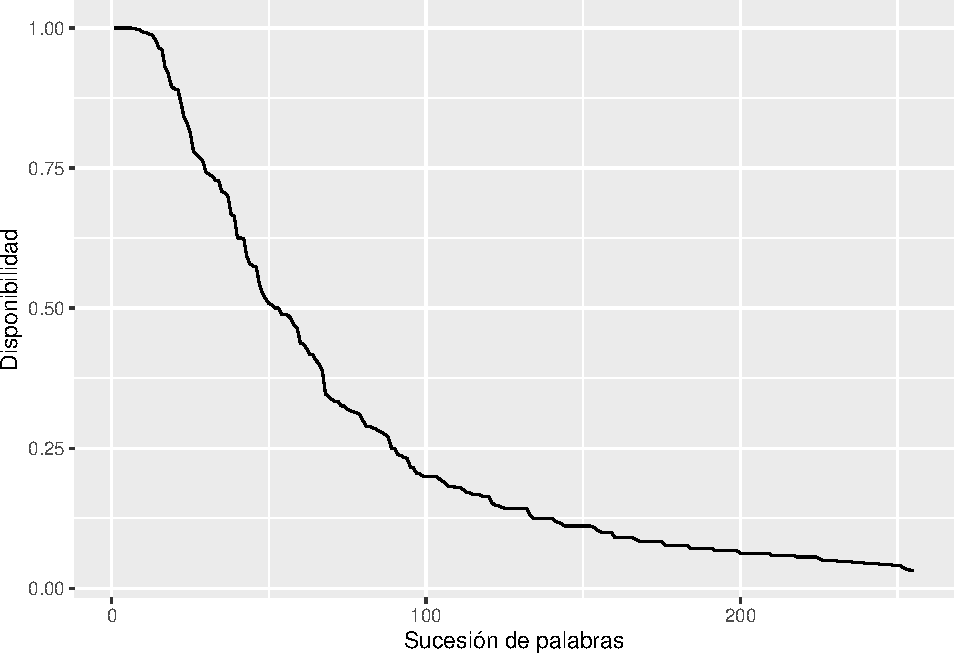
\includegraphics{PresentacionCentralex_files/figure-latex/unnamed-chunk-7-1.pdf}

\hypertarget{modelo-de-uxe1vila-suxe1nchez}{%
\subsection{Modelo de
Ávila-Sánchez}\label{modelo-de-uxe1vila-suxe1nchez}}

Ávila y Sánchez (2014 Fuzzy sets and Prototype Theory: Representational
model of cognitive community structures based on lexical availability
trials) propusieron un macro-modelo para el estudio de la disponibilidad
léxica a partir de la Teoría de los Conjuntos Difusos y mediante la
modelización de los conceptos que se pretenden representar. Esta
modelización se produce en dos etapas. En la primera, se cuantifica la
relevancia de cada término en las pruebas obtenidas para cada hablante y
centro de interés según una ley descendente según se avanza en cada
listado, y en la segunda etapa se integra esa información con una ley
aditiva que considera los distintos valores alcanzados para cada palabra
en cada centro de interés.

Hay múltiples posibles elecciones, pero en distintas pruebas resultaron
más prometedoras las que utilizaban en la primera etapa una ley de
Zipf-Mandelbrot y en la segunda una adición probabilística. La
interpretación de los valores obtenidos corresponde al concepto de
`centralidad' de cada término en cada centro de interés. Un valor de 1,
o muy cercano, respondería a la pertenencia al núcleo del vocabulario
específico del centro de interés, mientras que un valor próximo a 0
indicaría que se trataría de un término poco accesible y, por tanto,
descentralizado.

La función que lleva a cabo este análisis,
\texttt{build.avilasanchez.availability}, se utiliza de la misma forma
que la mostrada anteriormente en el modelo López-Strassburger:

\begin{Shaded}
\begin{Highlighting}[]
\NormalTok{disponibilidad <-}\StringTok{ }\KeywordTok{build.avilasanchez.availability}\NormalTok{(data)}
\end{Highlighting}
\end{Shaded}

El resultado es, de igual modo, un nuevo marco de datos con la
disponibilidad de cada término en cada centro de interés

\begin{Shaded}
\begin{Highlighting}[]
\NormalTok{disponibilidad }\OperatorTok\StringTok{ }
\StringTok{  }\KeywordTok{filter}\NormalTok{(centers}\OperatorTok{==}\StringTok{"03"}\NormalTok{) }\OperatorTok\StringTok{ }
\StringTok{  }\KeywordTok{arrange}\NormalTok{(}\OperatorTok{-}\NormalTok{availability) }\OperatorTok\StringTok{ }
\StringTok{  }\KeywordTok{head}\NormalTok{(}\DecValTok{10}\NormalTok{) }\OperatorTok\StringTok{ }
\StringTok{  }\KeywordTok{flextable}\NormalTok{() }\OperatorTok
\StringTok{  }\KeywordTok{set_header_labels}\NormalTok{(}\DataTypeTok{centers =} \StringTok{"Centro de interés"}\NormalTok{, }
                    \DataTypeTok{words=}\StringTok{"Palabra"}\NormalTok{, }
                    \DataTypeTok{order=}\StringTok{"Orden"}\NormalTok{, }
                    \DataTypeTok{availability=}\StringTok{"Disponibilidad"}\NormalTok{, }
                    \DataTypeTok{freq.abs=}\StringTok{"Frecuencia absoluta"}\NormalTok{, }
                    \DataTypeTok{freq.abs.cum=}\StringTok{"Frecuencia absoluta acumulada"}\NormalTok{, }
                    \DataTypeTok{freq.rel=}\StringTok{"Frecuencia relativa"}\NormalTok{, }
                    \DataTypeTok{freq.rel.cum=}\StringTok{"Frecuencia relativa acumulada"}\NormalTok{) }\OperatorTok
\StringTok{  }\KeywordTok{colformat_num}\NormalTok{(}\DataTypeTok{j=}\KeywordTok{c}\NormalTok{(}\DecValTok{4}\NormalTok{,}\DecValTok{6}\NormalTok{,}\DecValTok{8}\NormalTok{), }\DataTypeTok{digits=}\DecValTok{6}\NormalTok{) }\OperatorTok
\StringTok{  }\KeywordTok{width}\NormalTok{(}\DataTypeTok{j=}\KeywordTok{c}\NormalTok{(}\DecValTok{1}\NormalTok{,}\DecValTok{3}\NormalTok{,}\DecValTok{5}\NormalTok{,}\DecValTok{7}\NormalTok{),}\DataTypeTok{width=}\NormalTok{.}\DecValTok{65}\NormalTok{) }\OperatorTok
\StringTok{  }\KeywordTok{width}\NormalTok{(}\DataTypeTok{j=}\KeywordTok{c}\NormalTok{(}\DecValTok{2}\NormalTok{,}\DecValTok{4}\NormalTok{,}\DecValTok{6}\NormalTok{,}\DecValTok{8}\NormalTok{),}\DataTypeTok{width=}\NormalTok{.}\DecValTok{9}\NormalTok{) }\OperatorTok
\StringTok{  }\KeywordTok{theme_booktabs}\NormalTok{()}
\end{Highlighting}
\end{Shaded}

\begin{verbatim}
## PhantomJS not found. You can install it with webshot::install_phantomjs(). If it is installed, please make sure the phantomjs executable can be found via the PATH variable.
\end{verbatim}

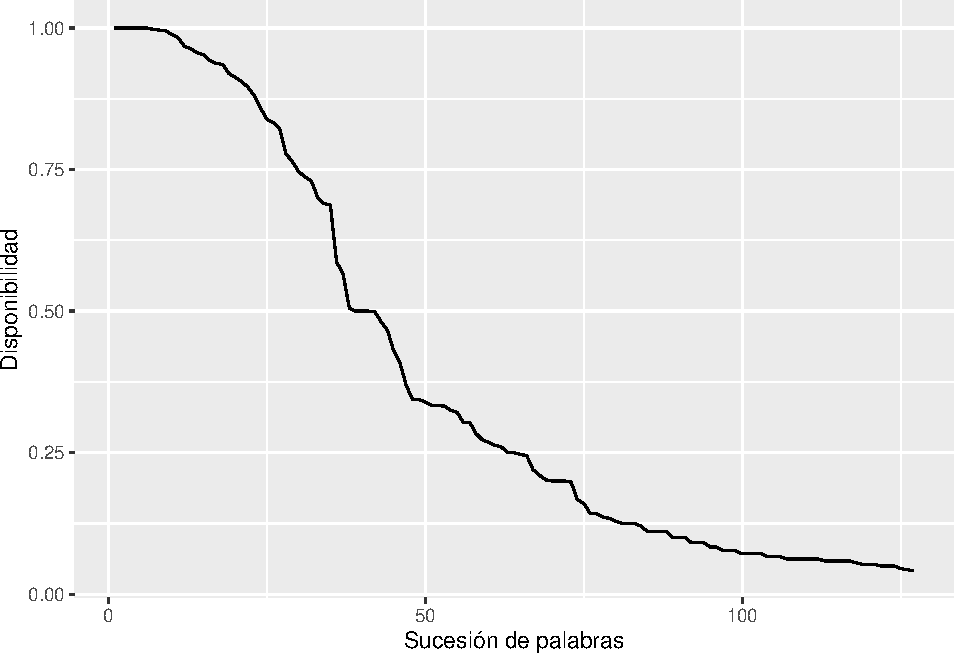
\includegraphics[width=6.20in,height=2.75in,keepaspectratio]{PresentacionCentralex_files/figure-latex/unnamed-chunk-9-1.png}
Que se puede procesar como cualquier marco de datos del sistema
\emph{R}:

\begin{Shaded}
\begin{Highlighting}[]
\NormalTok{disponibilidad }\OperatorTok\StringTok{ }
\StringTok{  }\KeywordTok{filter}\NormalTok{(centers}\OperatorTok{==}\StringTok{"03"}\NormalTok{) }\OperatorTok\StringTok{ }
\StringTok{  }\KeywordTok{arrange}\NormalTok{(}\OperatorTok{-}\NormalTok{availability) }\OperatorTok\StringTok{ }
\StringTok{  }\KeywordTok{ggplot}\NormalTok{(}\KeywordTok{aes}\NormalTok{(}\DataTypeTok{x=}\NormalTok{order, }\DataTypeTok{y=}\NormalTok{availability)) }\OperatorTok{+}\StringTok{ }\KeywordTok{geom_line}\NormalTok{() }\OperatorTok{+}
\StringTok{  }\KeywordTok{xlab}\NormalTok{(}\StringTok{"Sucesión de palabras"}\NormalTok{) }\OperatorTok{+}\StringTok{ }\KeywordTok{ylab}\NormalTok{(}\StringTok{"Disponibilidad"}\NormalTok{) }\OperatorTok{+}
\StringTok{  }\KeywordTok{theme_bw}\NormalTok{() }\OperatorTok{+}\StringTok{ }\KeywordTok{scale_colour_grey}\NormalTok{()}
\end{Highlighting}
\end{Shaded}

\includegraphics{PresentacionCentralex_files/figure-latex/unnamed-chunk-10-1.pdf}

Debido a las características de los operadores aditivos de la teoría de
los conjuntos difusos, es posible que la forma de la curva obtenida para
el cálculo de la disponibilidad clásica: quizás no aparezcan términos
con valores cercanos a 1 (por ejemplo, si se tienen pocos datos y estos
son relativamente dispersos) o, por el contrario, encontremos demasiados
términos con valoraciones cercanas a 1 (por ejemplo, si se trabaja con
muchas muestras). Aunque las opciones anteriores son improbables, pero
posibles, hemos optado por regular la curva mediante un parámetro
adicional, \texttt{k}, que va a modificar la curva
(ascendente-descendente), pero manteniendo su forma y clasificación. El
valor por defecto de \texttt{k} es 1. Si se da un valor entre 0 y 1, la
curva bajará (menos términos con valores cercanos a 1), mientras que si
a \texttt{k} se le da un valor mayor que la unidad la curva subirá (más
términos cercanos a la unidad).

\begin{Shaded}
\begin{Highlighting}[]
\NormalTok{disponibilidad <-}\StringTok{ }\KeywordTok{build.avilasanchez.availability}\NormalTok{(data, }\DataTypeTok{k =} \FloatTok{0.1}\NormalTok{)}
\NormalTok{disponibilidad }\OperatorTok
\StringTok{  }\KeywordTok{filter}\NormalTok{(centers}\OperatorTok{==}\StringTok{"03"}\NormalTok{) }\OperatorTok\StringTok{ }
\StringTok{  }\KeywordTok{arrange}\NormalTok{(}\OperatorTok{-}\NormalTok{availability) }\OperatorTok\StringTok{ }
\StringTok{  }\KeywordTok{ggplot}\NormalTok{(}\KeywordTok{aes}\NormalTok{(}\DataTypeTok{x=}\NormalTok{order, }\DataTypeTok{y=}\NormalTok{availability)) }\OperatorTok{+}\StringTok{ }\KeywordTok{geom_line}\NormalTok{() }\OperatorTok{+}
\StringTok{  }\KeywordTok{xlab}\NormalTok{(}\StringTok{"Sucesión de palabras"}\NormalTok{) }\OperatorTok{+}\StringTok{ }\KeywordTok{ylab}\NormalTok{(}\StringTok{"Disponibilidad"}\NormalTok{) }\OperatorTok{+}
\StringTok{  }\KeywordTok{theme_bw}\NormalTok{() }\OperatorTok{+}\StringTok{ }\KeywordTok{scale_colour_grey}\NormalTok{()}
\end{Highlighting}
\end{Shaded}

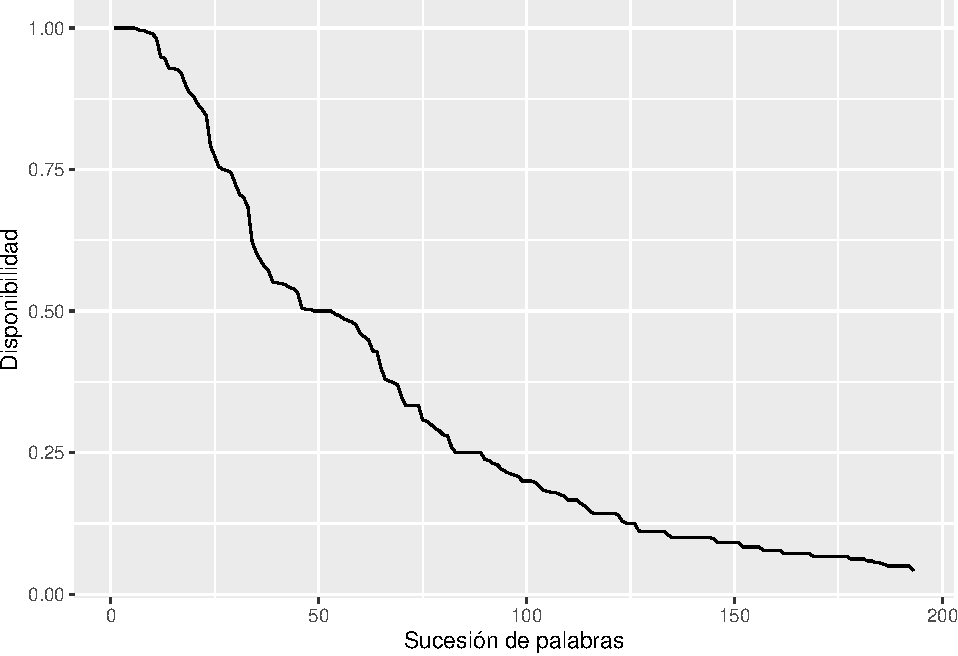
\includegraphics{PresentacionCentralex_files/figure-latex/unnamed-chunk-11-1.pdf}

El resultado final será, en cualquier caso, un nuevo marco de datos con
la disponibilidad de cada término en cada centro de interés

\begin{Shaded}
\begin{Highlighting}[]
\NormalTok{disponibilidad <-}\StringTok{ }\KeywordTok{build.avilasanchez.availability}\NormalTok{(data, }\DataTypeTok{k =} \DecValTok{2}\NormalTok{)}
\NormalTok{disponibilidad }\OperatorTok
\StringTok{  }\KeywordTok{filter}\NormalTok{(centers}\OperatorTok{==}\StringTok{"03"}\NormalTok{) }\OperatorTok\StringTok{ }
\StringTok{  }\KeywordTok{arrange}\NormalTok{(}\OperatorTok{-}\NormalTok{availability) }\OperatorTok\StringTok{ }
\StringTok{  }\KeywordTok{ggplot}\NormalTok{(}\KeywordTok{aes}\NormalTok{(}\DataTypeTok{x=}\KeywordTok{seq_along}\NormalTok{(availability), }\DataTypeTok{y=}\NormalTok{availability)) }\OperatorTok{+}\StringTok{ }\KeywordTok{geom_line}\NormalTok{() }\OperatorTok{+}
\StringTok{  }\KeywordTok{xlab}\NormalTok{(}\StringTok{"Sucesión de palabras"}\NormalTok{) }\OperatorTok{+}\StringTok{ }\KeywordTok{ylab}\NormalTok{(}\StringTok{"Disponibilidad"}\NormalTok{) }\OperatorTok{+}
\StringTok{  }\KeywordTok{theme_bw}\NormalTok{() }\OperatorTok{+}\StringTok{ }\KeywordTok{scale_colour_grey}\NormalTok{()}
\end{Highlighting}
\end{Shaded}

\includegraphics{PresentacionCentralex_files/figure-latex/unnamed-chunk-12-1.pdf}

Téngase en cuenta que los ejemplos mostrados representan de forma
artificial, manipulada y consciente, valores muy extremos usados a modo
de exposición. En nuestras pruebas, realizadas siempre con datos reales
procedentes de investigaciones previas, hemos encontrado que el valor de
referencia ofrece resultados adecuados en todos los casos que hemos
encontrado.

\hypertarget{niveles-de-disponibilidad}{%
\section{Niveles de disponibilidad}\label{niveles-de-disponibilidad}}

Una pregunta recurrente en casi todos los estudios previos de
disponibilidad léxica es considerar cuál es el tamaño del conjunto de
elementos que se habría que considerar para establecer el núcleo de un
centro de interés. Para responder a esta cuestión, y a partir del nuevo
marco teórico creado en nuestra propuesta, se proporciona una
herramienta que etiqueta los términos por niveles de centralidad. El
nivel 0 correspondería a aquellos elementos que no pertenecen al núcleo,
es decir, aquellos términos que no son generalmente accesibles. Los
níveles 1, 2, 3, \ldots{} y sucesivos representarían un mayor grado de
centralidad y aproximación al centro de interés.

\begin{Shaded}
\begin{Highlighting}[]
\NormalTok{disponibilidad <-}\StringTok{ }\KeywordTok{build.avilasanchez.availability}\NormalTok{(data)}
\NormalTok{levels <-}\StringTok{ }\KeywordTok{classify.availability.levels}\NormalTok{(disponibilidad)}
\NormalTok{levels }\OperatorTok\StringTok{ }
\StringTok{  }\KeywordTok{head}\NormalTok{(}\DecValTok{20}\NormalTok{) }\OperatorTok
\StringTok{  }\KeywordTok{arrange}\NormalTok{(}\OperatorTok{-}\NormalTok{availability) }\OperatorTok
\StringTok{  }\KeywordTok{select}\NormalTok{(}\OperatorTok{-}\NormalTok{order) }\OperatorTok
\StringTok{  }\KeywordTok{flextable}\NormalTok{() }\OperatorTok
\StringTok{  }\KeywordTok{set_header_labels}\NormalTok{(}\DataTypeTok{centers =} \StringTok{"Centro de interés"}\NormalTok{, }
                    \DataTypeTok{words=}\StringTok{"Palabra"}\NormalTok{, }
                    \DataTypeTok{availability=}\StringTok{"Disponibilidad"}\NormalTok{,}
                    \DataTypeTok{level=}\StringTok{"Nivel de disponibilidad"}\NormalTok{,}
                    \DataTypeTok{cutlevel=}\StringTok{"Nivel de corte"}\NormalTok{,}
                    \DataTypeTok{freq.abs=}\StringTok{"Frecuencia absoluta"}\NormalTok{, }
                    \DataTypeTok{freq.abs.cum=}\StringTok{"Frecuencia absoluta acumulada"}\NormalTok{, }
                    \DataTypeTok{freq.rel=}\StringTok{"Frecuencia relativa"}\NormalTok{, }
                    \DataTypeTok{freq.rel.cum=}\StringTok{"Frecuencia relativa acumulada"}\NormalTok{) }\OperatorTok
\StringTok{  }\KeywordTok{colformat_num}\NormalTok{(}\DataTypeTok{j=}\KeywordTok{c}\NormalTok{(}\DecValTok{5}\NormalTok{,}\DecValTok{7}\NormalTok{,}\DecValTok{9}\NormalTok{), }\DataTypeTok{digits=}\DecValTok{5}\NormalTok{) }\OperatorTok
\StringTok{  }\KeywordTok{width}\NormalTok{(}\DataTypeTok{j=}\KeywordTok{c}\NormalTok{(}\DecValTok{1}\NormalTok{,}\DecValTok{4}\NormalTok{,}\DecValTok{6}\NormalTok{,}\DecValTok{8}\NormalTok{),}\DataTypeTok{width=}\NormalTok{.}\DecValTok{65}\NormalTok{) }\OperatorTok
\StringTok{  }\KeywordTok{width}\NormalTok{(}\DataTypeTok{j=}\KeywordTok{c}\NormalTok{(}\DecValTok{2}\NormalTok{,}\DecValTok{3}\NormalTok{,}\DecValTok{5}\NormalTok{,}\DecValTok{6}\NormalTok{,}\DecValTok{7}\NormalTok{,}\DecValTok{9}\NormalTok{),}\DataTypeTok{width=}\NormalTok{.}\DecValTok{75}\NormalTok{) }\OperatorTok
\StringTok{  }\KeywordTok{theme_booktabs}\NormalTok{()}
\end{Highlighting}
\end{Shaded}

\begin{verbatim}
## PhantomJS not found. You can install it with webshot::install_phantomjs(). If it is installed, please make sure the phantomjs executable can be found via the PATH variable.
\end{verbatim}

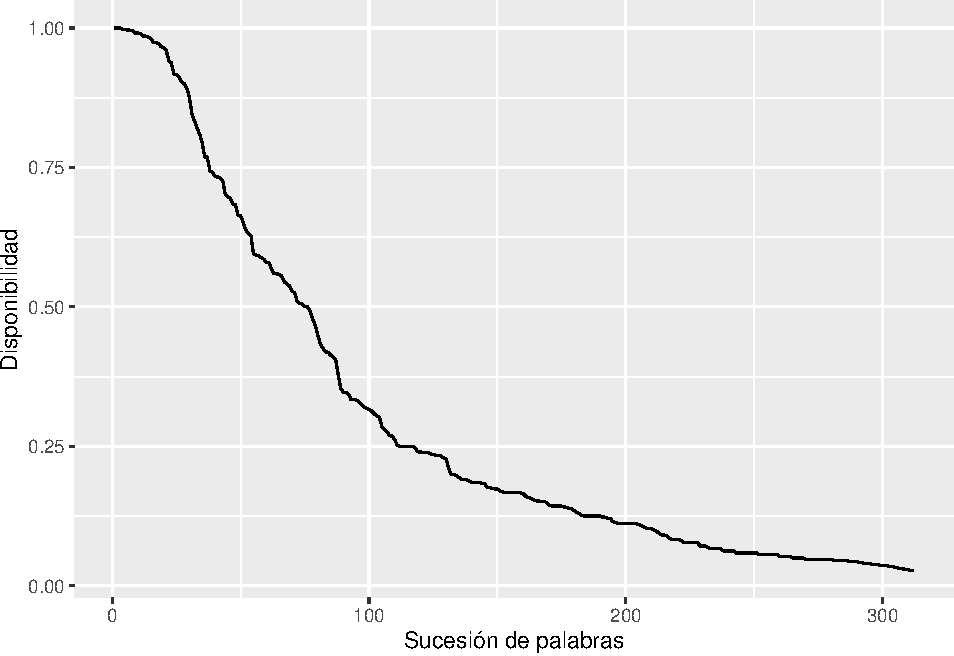
\includegraphics[width=6.45in,height=5.25in,keepaspectratio]{PresentacionCentralex_files/figure-latex/unnamed-chunk-13-1.png}

\begin{Shaded}
\begin{Highlighting}[]
\NormalTok{levels }\OperatorTok\StringTok{ }
\StringTok{  }\KeywordTok{filter}\NormalTok{(centers}\OperatorTok{==}\StringTok{"01"}\NormalTok{) }\OperatorTok\StringTok{ }
\StringTok{  }\KeywordTok{arrange}\NormalTok{(}\OperatorTok{-}\NormalTok{availability)   }\OperatorTok\StringTok{ }
\StringTok{  }\KeywordTok{filter}\NormalTok{(level }\OperatorTok{>}\StringTok{ }\DecValTok{0}\NormalTok{) }\OperatorTok
\StringTok{  }\KeywordTok{select}\NormalTok{(}\OperatorTok{-}\NormalTok{order) }\OperatorTok\StringTok{ }
\StringTok{  }\KeywordTok{flextable}\NormalTok{() }\OperatorTok\StringTok{ }
\StringTok{  }\KeywordTok{set_header_labels}\NormalTok{(}\DataTypeTok{centers =} \StringTok{"Centro de interés"}\NormalTok{, }
                    \DataTypeTok{words=}\StringTok{"Palabra"}\NormalTok{, }
                    \DataTypeTok{availability=}\StringTok{"Disponibilidad"}\NormalTok{,}
                    \DataTypeTok{level=}\StringTok{"Nivel de disponibilidad"}\NormalTok{,}
                    \DataTypeTok{cutlevel=}\StringTok{"Nivel de corte"}\NormalTok{,}
                    \DataTypeTok{freq.abs=}\StringTok{"Frecuencia absoluta"}\NormalTok{, }
                    \DataTypeTok{freq.abs.cum=}\StringTok{"Frecuencia absoluta acumulada"}\NormalTok{, }
                    \DataTypeTok{freq.rel=}\StringTok{"Frecuencia relativa"}\NormalTok{, }
                    \DataTypeTok{freq.rel.cum=}\StringTok{"Frecuencia relativa acumulada"}\NormalTok{) }\OperatorTok
\StringTok{  }\KeywordTok{colformat_num}\NormalTok{(}\DataTypeTok{j=}\KeywordTok{c}\NormalTok{(}\DecValTok{3}\NormalTok{,}\DecValTok{5}\NormalTok{,}\DecValTok{7}\NormalTok{,}\DecValTok{9}\NormalTok{), }\DataTypeTok{digits=}\DecValTok{5}\NormalTok{) }\OperatorTok
\StringTok{  }\KeywordTok{width}\NormalTok{(}\DataTypeTok{j=}\KeywordTok{c}\NormalTok{(}\DecValTok{1}\NormalTok{,}\DecValTok{4}\NormalTok{,}\DecValTok{6}\NormalTok{,}\DecValTok{8}\NormalTok{),}\DataTypeTok{width=}\NormalTok{.}\DecValTok{65}\NormalTok{) }\OperatorTok
\StringTok{  }\KeywordTok{width}\NormalTok{(}\DataTypeTok{j=}\KeywordTok{c}\NormalTok{(}\DecValTok{2}\NormalTok{,}\DecValTok{3}\NormalTok{,}\DecValTok{5}\NormalTok{,}\DecValTok{6}\NormalTok{,}\DecValTok{7}\NormalTok{,}\DecValTok{9}\NormalTok{),}\DataTypeTok{width=}\NormalTok{.}\DecValTok{75}\NormalTok{) }\OperatorTok
\StringTok{  }\KeywordTok{theme_booktabs}\NormalTok{()}
\end{Highlighting}
\end{Shaded}

\begin{verbatim}
## PhantomJS not found. You can install it with webshot::install_phantomjs(). If it is installed, please make sure the phantomjs executable can be found via the PATH variable.
\end{verbatim}

\includegraphics[width=6.45in,height=15.00in,keepaspectratio]{PresentacionCentralex_files/figure-latex/unnamed-chunk-14-1.png}

Con esta información se puede construir una representación en la que se
observa la distribución de las disponibilidades en el centro de interés
y los diferentes conjuntos de cortes.

\begin{Shaded}
\begin{Highlighting}[]
\NormalTok{levels }\OperatorTok
\StringTok{  }\KeywordTok{filter}\NormalTok{(centers}\OperatorTok{==}\StringTok{"04"}\NormalTok{) }\OperatorTok\StringTok{ }
\StringTok{  }\KeywordTok{mutate}\NormalTok{(}\DataTypeTok{level=}\KeywordTok{factor}\NormalTok{(level)) }\OperatorTok\StringTok{ }
\StringTok{  }\KeywordTok{arrange}\NormalTok{(}\OperatorTok{-}\NormalTok{availability) }\OperatorTok\StringTok{ }
\StringTok{  }\KeywordTok{ggplot}\NormalTok{(}\KeywordTok{aes}\NormalTok{(}\DataTypeTok{x=}\NormalTok{order,}\DataTypeTok{y=}\NormalTok{availability,}\DataTypeTok{color=}\NormalTok{level)) }\OperatorTok{+}\StringTok{ }\KeywordTok{geom_line}\NormalTok{() }\OperatorTok{+}
\StringTok{  }\KeywordTok{xlab}\NormalTok{(}\StringTok{"Posición del término en el centro de interés"}\NormalTok{) }\OperatorTok{+}
\StringTok{  }\KeywordTok{ylab}\NormalTok{(}\StringTok{"Disponibilidad"}\NormalTok{) }\OperatorTok{+}
\StringTok{  }\KeywordTok{theme_bw}\NormalTok{() }\OperatorTok{+}\StringTok{ }\KeywordTok{scale_colour_grey}\NormalTok{()}
\end{Highlighting}
\end{Shaded}

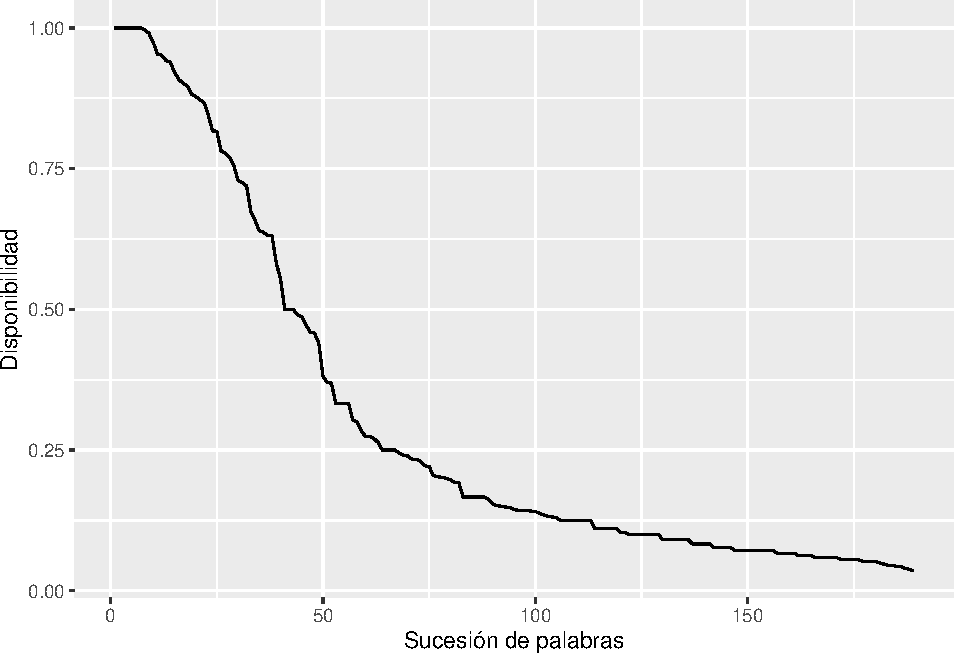
\includegraphics{PresentacionCentralex_files/figure-latex/unnamed-chunk-15-1.pdf}

Se han construido utilidades para ayudar a la representación de estos
conjuntos de cortes. El siguiente ejemplo muestra los principales
conjuntos de corte obtenidos en los 16 centros de interés usados en el
trabajo de Villena Ponsoda y Ávila Muñoz (2010)

\begin{Shaded}
\begin{Highlighting}[]
\NormalTok{clasificacion <-}\StringTok{ }\KeywordTok{build.availability.levels}\NormalTok{(levels)}
\NormalTok{clasificacion }\OperatorTok\StringTok{ }
\StringTok{  }\KeywordTok{filter}\NormalTok{(level}\OperatorTok{>}\StringTok{ }\DecValTok{0}\NormalTok{)  }\OperatorTok
\StringTok{  }\KeywordTok{flextable}\NormalTok{() }\OperatorTok\StringTok{ }
\StringTok{  }\KeywordTok{set_header_labels}\NormalTok{(}\DataTypeTok{centers =} \StringTok{"Centro de interés"}\NormalTok{, }
                    \DataTypeTok{words=}\StringTok{"Palabras"}\NormalTok{, }
                    \DataTypeTok{level=}\StringTok{"Nivel de disponibilidad"}\NormalTok{,}
                    \DataTypeTok{count=}\StringTok{"Recuento"}\NormalTok{) }\OperatorTok
\StringTok{  }\KeywordTok{width}\NormalTok{(}\DataTypeTok{j=}\KeywordTok{c}\NormalTok{(}\DecValTok{1}\NormalTok{,}\DecValTok{2}\NormalTok{,}\DecValTok{3}\NormalTok{),}\DataTypeTok{width=}\NormalTok{.}\DecValTok{75}\NormalTok{) }\OperatorTok
\StringTok{  }\KeywordTok{width}\NormalTok{(}\DataTypeTok{j=}\DecValTok{4}\NormalTok{,}\DataTypeTok{width=}\DecValTok{4}\NormalTok{) }\OperatorTok
\StringTok{  }\KeywordTok{align}\NormalTok{(}\DataTypeTok{i=}\DecValTok{4}\NormalTok{,}\DataTypeTok{align=}\StringTok{"right"}\NormalTok{) }\OperatorTok
\StringTok{  }\KeywordTok{theme_booktabs}\NormalTok{()}
\end{Highlighting}
\end{Shaded}

\begin{verbatim}
## PhantomJS not found. You can install it with webshot::install_phantomjs(). If it is installed, please make sure the phantomjs executable can be found via the PATH variable.
\end{verbatim}

\includegraphics[width=6.25in,height=30.25in,keepaspectratio]{PresentacionCentralex_files/figure-latex/unnamed-chunk-16-1.png}

\begin{Shaded}
\begin{Highlighting}[]
\NormalTok{levels }\OperatorTok
\StringTok{  }\KeywordTok{mutate}\NormalTok{(}\DataTypeTok{level=}\KeywordTok{factor}\NormalTok{(level)) }\OperatorTok\StringTok{ }
\StringTok{  }\KeywordTok{filter}\NormalTok{(centers }\OperatorTok\StringTok{ }\KeywordTok{c}\NormalTok{(}\StringTok{"01"}\NormalTok{,}\StringTok{"02"}\NormalTok{,}\StringTok{"03"}\NormalTok{,}\StringTok{"04"}\NormalTok{)) }\OperatorTok
\StringTok{  }\KeywordTok{arrange}\NormalTok{(}\OperatorTok{-}\NormalTok{availability) }\OperatorTok\StringTok{ }
\StringTok{  }\KeywordTok{ggplot}\NormalTok{(}\KeywordTok{aes}\NormalTok{(}\DataTypeTok{x=}\NormalTok{order,}\DataTypeTok{y=}\NormalTok{availability,}\DataTypeTok{color=}\NormalTok{level)) }\OperatorTok{+}\StringTok{ }\KeywordTok{geom_line}\NormalTok{() }\OperatorTok{+}\StringTok{ }\KeywordTok{facet_wrap}\NormalTok{(}\OperatorTok{~}\NormalTok{centers)  }\OperatorTok{+}
\StringTok{  }\KeywordTok{xlab}\NormalTok{(}\StringTok{"Secuencia de palabras (por grado descendente de compatibilidad)"}\NormalTok{) }\OperatorTok{+}\StringTok{ }
\StringTok{  }\KeywordTok{ylab}\NormalTok{(}\StringTok{"Disponibilidad"}\NormalTok{) }\OperatorTok{+}
\StringTok{  }\KeywordTok{theme_bw}\NormalTok{() }\OperatorTok{+}\StringTok{ }\KeywordTok{scale_colour_grey}\NormalTok{()}
\end{Highlighting}
\end{Shaded}

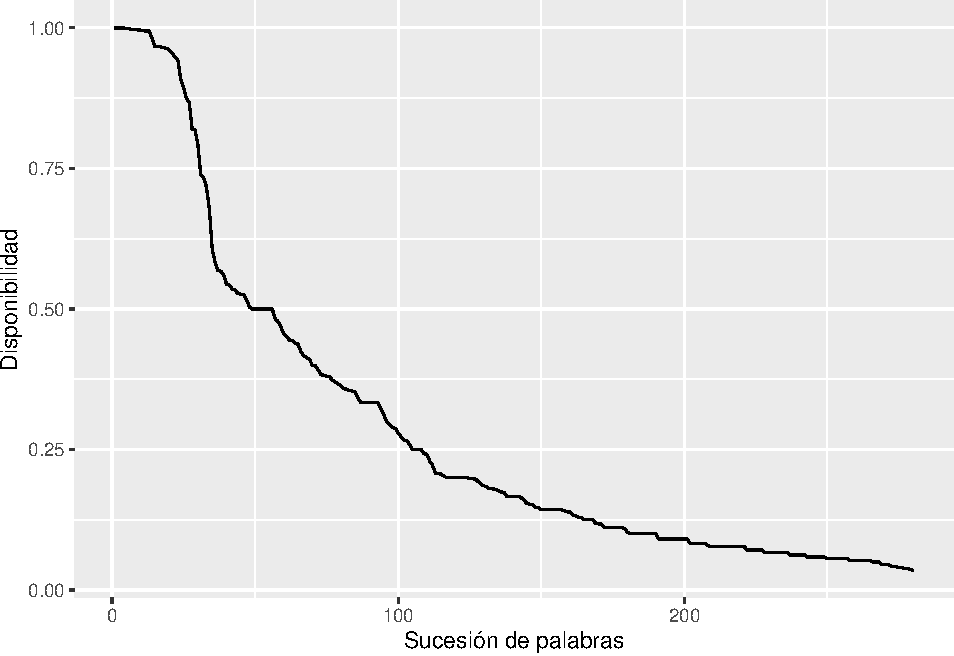
\includegraphics{PresentacionCentralex_files/figure-latex/unnamed-chunk-17-1.pdf}

\hypertarget{herramienta-propuesta}{%
\section{Herramienta propuesta}\label{herramienta-propuesta}}

Para facilitar el acceso a esta herramienta se ha dispuesto una pequeña
utilidad gráfica que construye un documento básico con construcciones
que opinamos que cubren las necesidades generales para el estudio de la
disponibilidad. Este documento puede ser fácilmente modificable para
adaptarlo a las necesidades de cada usuario.

Incluyendo la carga de la librería se puede invocar como:

\begin{Shaded}
\begin{Highlighting}[]
\KeywordTok{library}\NormalTok{(dispocen)}
\NormalTok{dispocen}\OperatorTok{::}\KeywordTok{runUtility}\NormalTok{()}
\end{Highlighting}
\end{Shaded}

abriéndose un interfaz gráfico con el siguiente aspecto:
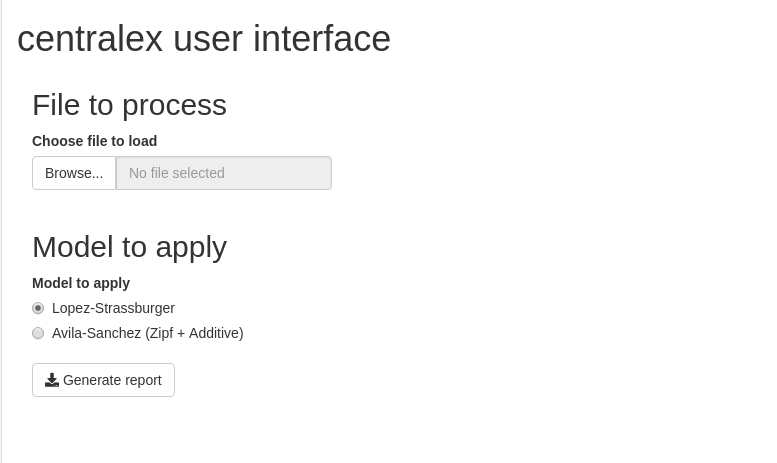
\includegraphics{imgs/dispocen01.png} Proporcionado un archivo de datos,
seleccionado el modelo de procesamiento (inicialmente se proporcionan
dos opciones, el modelo de disponibilidad propuesto por
López-Strassburger y el de centralidad propuesto por Ávila-Sánchez) se
confirman los datos y se ofrece la descarga de un documento que ha de
guardarse junto al archivo de datos.

Este documento incluye los bloques de código que llevan a cabo los
procedimientos que hemos considerado útiles y que ofrecen sus resultados
en el formato expuesto en este trabajo. Muchos bloques están etiquetados
con la opción \texttt{eval=FALSE}, que hace que no se ejecuten por
defecto. Si se está interesado en los resultados correspondientes, tan
sólo hay que eliminar esa opción.

Se proporcionan las siguientes secciones:

\begin{itemize}
\tightlist
\item
  Carga de datos y modelo de disponibilidad: estas secciones son
  imprescindibles, o no se podría lleva a cabo el análisis. Se
  proporcionan una serie de bloques que permiten exponer los datos
  obtenidos por centro de interés, en forma de tabla y de gráfico, y un
  resumen gráfico de todos los centros de interés.
\item
  Niveles de centralidad/disponibilidad: se clasifican las palabras por
  niveles y se construyen los listados de términos por nivel. Se
  posibilita obtener los listados con la clasificación y otros datos
  asociados y las tablas resumen. Se han habilitado por defecto la
  presentación de los niveles de los términos por encima del nivel
  básico, de menor centralidad.
\end{itemize}

Nótese que este documento es un documento RMarkdown que es fácilmente
modificable y personalizable. Se procesa entonces, dando lugar a un
documento PDF, Word o HTML, entre otras opciones, que puede utilizarse
como base para completar el trabajo.

\hypertarget{ejemplos-de-uso}{%
\section{Ejemplos de uso}\label{ejemplos-de-uso}}

Hemos decidido, de forma predeterminada, no considerar el uso de las
primeras columnas para datos sociológicos en los datos porque su
limitado formato y redundancia no constituye una buena práctica,
siguiendo los criterios de la normalización de bases de datos y de
análisis de datos.

Así, presentamos algunas propuestas que consideramos más productivas
para llevar a cabo estos datos.

\hypertarget{los-datos-socioluxf3gicos}{%
\subsection{Los datos sociológicos}\label{los-datos-socioluxf3gicos}}

En primer lugar, es importante evitar la redundancia de los datos, tanto
por la dificultad que implica mantener la coherencia de los mismos
cuando se encuentran duplicados en varios lugares como por facilitar
mantenerlos actualizados.

\begin{Shaded}
\begin{Highlighting}[]
\NormalTok{bs <-}\StringTok{ }\KeywordTok{read.csv}\NormalTok{(}\StringTok{"BaseSociologica.csv"}\NormalTok{, }\DataTypeTok{colClasses =} \StringTok{"character"}\NormalTok{)}
\NormalTok{bs <-}\StringTok{ }\NormalTok{bs }\OperatorTok
\StringTok{  }\KeywordTok{mutate}\NormalTok{(}\DataTypeTok{EDAD=}\KeywordTok{strtoi}\NormalTok{(EDAD),}
\NormalTok{         AÑ}\DataTypeTok{OSDEESTUDIO =} \KeywordTok{strtoi}\NormalTok{(AÑOSDEESTUDIO))}
\end{Highlighting}
\end{Shaded}

\begin{Shaded}
\begin{Highlighting}[]
\NormalTok{bs }\OperatorTok
\StringTok{  }\KeywordTok{head}\NormalTok{()  }\OperatorTok
\StringTok{  }\KeywordTok{select}\NormalTok{(SUJETO,SEXO,EDAD,AÑOSDEESTUDIO) }\OperatorTok
\StringTok{  }\KeywordTok{flextable}\NormalTok{() }\OperatorTok
\StringTok{  }\KeywordTok{autofit}\NormalTok{()}
\end{Highlighting}
\end{Shaded}

\begin{verbatim}
## PhantomJS not found. You can install it with webshot::install_phantomjs(). If it is installed, please make sure the phantomjs executable can be found via the PATH variable.
\end{verbatim}

\includegraphics[width=3.67in,height=2.03in,keepaspectratio]{PresentacionCentralex_files/figure-latex/unnamed-chunk-20-1.png}

\hypertarget{anuxe1lisis-separados-por-sexo}{%
\subsection{Análisis separados por
sexo}\label{anuxe1lisis-separados-por-sexo}}

Si se desea llevar a cabo un análisis de centralidad léxica, separados
por sexos, se pretende llevar a cabo la integración de la información
proporcionada por hombres y mujeres. Así que se filtrarían las
realizaciones a procesar seleccionando a los sujetos que cumplen esas
características:

\begin{Shaded}
\begin{Highlighting}[]
\NormalTok{idHombres <-}
\StringTok{  }\NormalTok{bs }\OperatorTok\StringTok{ }
\StringTok{  }\KeywordTok{filter}\NormalTok{(SEXO}\OperatorTok{==}\StringTok{"1"}\NormalTok{) }\OperatorTok
\StringTok{  }\KeywordTok{select}\NormalTok{(SUJETO) }\OperatorTok
\StringTok{  }\KeywordTok{unlist}\NormalTok{()}
\NormalTok{idHombres}
\end{Highlighting}
\end{Shaded}

\begin{verbatim}
##  SUJETO1  SUJETO2  SUJETO3  SUJETO4  SUJETO5  SUJETO6  SUJETO7  SUJETO8 
##    "001"    "004"    "006"    "010"    "012"    "014"    "015"    "022" 
##  SUJETO9 SUJETO10 SUJETO11 SUJETO12 SUJETO13 SUJETO14 SUJETO15 SUJETO16 
##    "026"    "029"    "032"    "035"    "036"    "039"    "041"    "043" 
## SUJETO17 SUJETO18 SUJETO19 SUJETO20 SUJETO21 SUJETO22 SUJETO23 SUJETO24 
##    "046"    "049"    "050"    "051"    "052"    "053"    "055"    "058" 
## SUJETO25 SUJETO26 SUJETO27 SUJETO28 SUJETO29 SUJETO30 SUJETO31 SUJETO32 
##    "061"    "064"    "065"    "070"    "073"    "075"    "076"    "097" 
## SUJETO33 SUJETO34 
##    "098"    "099"
\end{verbatim}

\begin{Shaded}
\begin{Highlighting}[]
\NormalTok{idMujeres <-}
\StringTok{  }\NormalTok{bs }\OperatorTok\StringTok{ }
\StringTok{  }\KeywordTok{filter}\NormalTok{(SEXO}\OperatorTok{==}\StringTok{"0"}\NormalTok{) }\OperatorTok
\StringTok{  }\KeywordTok{select}\NormalTok{(SUJETO) }\OperatorTok
\StringTok{  }\KeywordTok{unlist}\NormalTok{()}
\NormalTok{idMujeres}
\end{Highlighting}
\end{Shaded}

\begin{verbatim}
##  SUJETO1  SUJETO2  SUJETO3  SUJETO4  SUJETO5  SUJETO6  SUJETO7  SUJETO8 
##    "002"    "003"    "005"    "008"    "009"    "013"    "019"    "021" 
##  SUJETO9 SUJETO10 SUJETO11 SUJETO12 SUJETO13 SUJETO14 SUJETO15 SUJETO16 
##    "023"    "024"    "025"    "027"    "028"    "030"    "031"    "033" 
## SUJETO17 SUJETO18 SUJETO19 SUJETO20 SUJETO21 SUJETO22 SUJETO23 SUJETO24 
##    "034"    "037"    "038"    "040"    "042"    "045"    "047"    "048" 
## SUJETO25 SUJETO26 SUJETO27 SUJETO28 SUJETO29 SUJETO30 SUJETO31 SUJETO32 
##    "056"    "059"    "060"    "062"    "063"    "066"    "067"    "068" 
## SUJETO33 SUJETO34 SUJETO35 SUJETO36 SUJETO37 SUJETO38 
##    "069"    "071"    "072"    "074"    "077"    "096"
\end{verbatim}

Entonces, se pueden separar las realizaciones, si los sujetos pertenecen
al grupo de hombres o mujeres

\begin{Shaded}
\begin{Highlighting}[]
\NormalTok{data }\OperatorTok\StringTok{ }
\StringTok{  }\KeywordTok{filter}\NormalTok{(users }\OperatorTok\StringTok{ }\NormalTok{idMujeres) }\OperatorTok
\StringTok{  }\KeywordTok{head}\NormalTok{()}
\end{Highlighting}
\end{Shaded}

\begin{verbatim}
##   infos users centers        words
## 1 12131   002      01 riñón, c....
## 2 12213   003      01 brazo, m....
## 3 12214   005      01 cabeza, ....
## 4 11232   008      01 cabeza, ....
## 5 11221   009      01 músculo,....
## 6 12224   013      01 cabeza, ....
\end{verbatim}

\begin{Shaded}
\begin{Highlighting}[]
\NormalTok{data }\OperatorTok\StringTok{ }
\StringTok{  }\KeywordTok{filter}\NormalTok{(users }\OperatorTok\StringTok{ }\NormalTok{idHombres) }\OperatorTok
\StringTok{  }\KeywordTok{head}\NormalTok{()}
\end{Highlighting}
\end{Shaded}

\begin{verbatim}
##   infos users centers        words
## 1 21131   001      01 mano, pi....
## 2 22214   004      01 brazo, o....
## 3 22213   006      01 pie, man....
## 4 22224   010      01 esquelet....
## 5 22224   012      01 cabeza, ....
## 6 22212   014      01 mano, pi....
\end{verbatim}

Y se pueden procesar de la forma habitual:

\begin{Shaded}
\begin{Highlighting}[]
\NormalTok{disponibilidadHombres <-}\StringTok{ }
\StringTok{  }\KeywordTok{build.avilasanchez.availability}\NormalTok{(data }\OperatorTok
\StringTok{                                  }\KeywordTok{filter}\NormalTok{(users }\OperatorTok\StringTok{ }\NormalTok{idHombres))}
\KeywordTok{head}\NormalTok{(disponibilidadHombres) }\OperatorTok
\StringTok{  }\KeywordTok{select}\NormalTok{(centers, words, availability) }\OperatorTok
\StringTok{  }\KeywordTok{flextable}\NormalTok{() }\OperatorTok
\StringTok{  }\KeywordTok{autofit}\NormalTok{()}
\end{Highlighting}
\end{Shaded}

\begin{verbatim}
## PhantomJS not found. You can install it with webshot::install_phantomjs(). If it is installed, please make sure the phantomjs executable can be found via the PATH variable.
\end{verbatim}

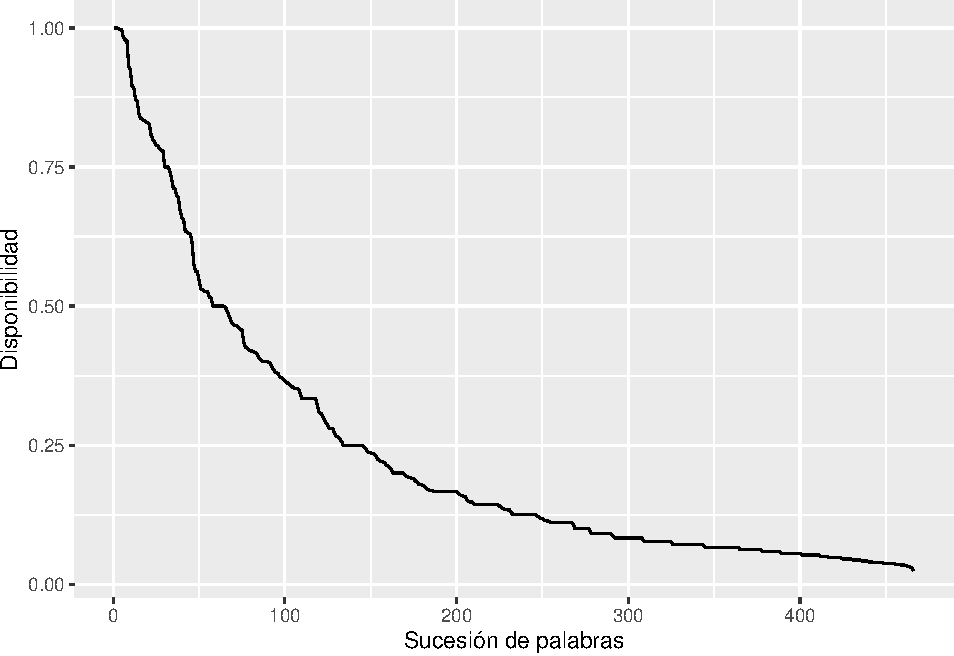
\includegraphics[width=2.58in,height=2.13in,keepaspectratio]{PresentacionCentralex_files/figure-latex/unnamed-chunk-25-1.png}

\begin{Shaded}
\begin{Highlighting}[]
\NormalTok{disponibilidadMujeres <-}\StringTok{ }
\StringTok{  }\KeywordTok{build.avilasanchez.availability}\NormalTok{(data }\OperatorTok
\StringTok{                                  }\KeywordTok{filter}\NormalTok{(users }\OperatorTok\StringTok{ }\NormalTok{idMujeres))}
\KeywordTok{head}\NormalTok{(disponibilidadMujeres) }\OperatorTok
\StringTok{  }\KeywordTok{select}\NormalTok{(centers, words, availability) }\OperatorTok
\StringTok{  }\KeywordTok{flextable}\NormalTok{() }\OperatorTok
\StringTok{  }\KeywordTok{autofit}\NormalTok{()}
\end{Highlighting}
\end{Shaded}

\begin{verbatim}
## PhantomJS not found. You can install it with webshot::install_phantomjs(). If it is installed, please make sure the phantomjs executable can be found via the PATH variable.
\end{verbatim}

\includegraphics[width=2.58in,height=2.13in,keepaspectratio]{PresentacionCentralex_files/figure-latex/unnamed-chunk-26-1.png}
Esta información se puede combinar para realizar análisis comparativos,
enlazando los datos por centros de interés y términos

\begin{Shaded}
\begin{Highlighting}[]
\NormalTok{dispComp <-}
\StringTok{  }\KeywordTok{inner_join}\NormalTok{(disponibilidadHombres }\OperatorTok\StringTok{ }
\StringTok{             }\KeywordTok{select}\NormalTok{(centers,words,availability) }\OperatorTok
\StringTok{             }\KeywordTok{rename}\NormalTok{(}\DataTypeTok{avHombres=}\NormalTok{availability), }
\NormalTok{             disponibilidadMujeres }\OperatorTok
\StringTok{             }\KeywordTok{select}\NormalTok{(centers,words,availability) }\OperatorTok
\StringTok{             }\KeywordTok{rename}\NormalTok{(}\DataTypeTok{avMujeres=}\NormalTok{availability),}
           \DataTypeTok{by =} \KeywordTok{c}\NormalTok{(}\StringTok{"centers"}\NormalTok{, }\StringTok{"words"}\NormalTok{))}
\NormalTok{dispComp }\OperatorTok
\StringTok{  }\KeywordTok{head}\NormalTok{() }\OperatorTok
\StringTok{  }\KeywordTok{flextable}\NormalTok{() }\OperatorTok
\StringTok{  }\KeywordTok{autofit}\NormalTok{()}
\end{Highlighting}
\end{Shaded}

\begin{verbatim}
## PhantomJS not found. You can install it with webshot::install_phantomjs(). If it is installed, please make sure the phantomjs executable can be found via the PATH variable.
\end{verbatim}

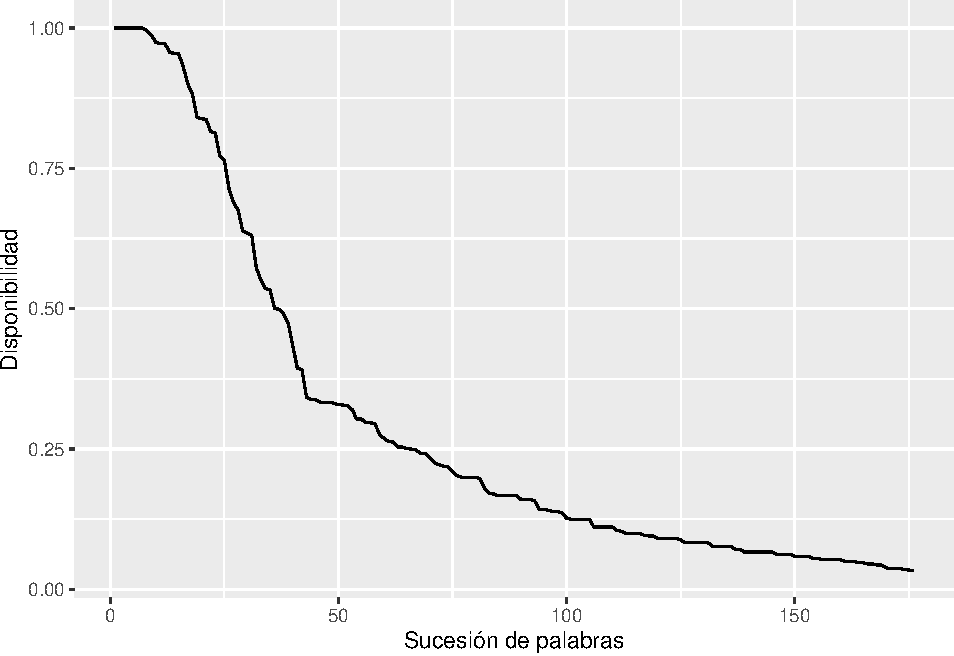
\includegraphics[width=3.65in,height=2.13in,keepaspectratio]{PresentacionCentralex_files/figure-latex/unnamed-chunk-27-1.png}

\begin{Shaded}
\begin{Highlighting}[]
\NormalTok{dispComp }\OperatorTok
\StringTok{  }\KeywordTok{ggplot}\NormalTok{(}\KeywordTok{aes}\NormalTok{(}\DataTypeTok{x=}\NormalTok{avHombres,}\DataTypeTok{y=}\NormalTok{avMujeres,}\DataTypeTok{color=}\NormalTok{centers)) }\OperatorTok{+}\StringTok{ }\KeywordTok{geom_point}\NormalTok{() }\OperatorTok{+}
\StringTok{  }\KeywordTok{theme_bw}\NormalTok{() }\OperatorTok{+}\StringTok{ }\KeywordTok{scale_colour_grey}\NormalTok{()}
\end{Highlighting}
\end{Shaded}

\includegraphics{PresentacionCentralex_files/figure-latex/unnamed-chunk-28-1.pdf}

Según este gráfico es posible observar que los términos muy disponibles
y poco disponibles tienden a ser similares. Sin embargo, los términos
que aparecen en los diversos niveles intermedios pueden variar de forma
muy significativa.

\begin{Shaded}
\begin{Highlighting}[]
\NormalTok{levelsHombres <-}\StringTok{ }\KeywordTok{classify.availability.levels}\NormalTok{(disponibilidadHombres)}
\NormalTok{clasificacionHombres <-}\StringTok{ }\KeywordTok{build.availability.levels}\NormalTok{(levelsHombres)}
\NormalTok{levelsMujeres <-}\StringTok{ }\KeywordTok{classify.availability.levels}\NormalTok{(disponibilidadMujeres)}
\NormalTok{clasificacionMujeres <-}\StringTok{ }\KeywordTok{build.availability.levels}\NormalTok{(levelsMujeres)}
\NormalTok{clasificacionSexo <-}
\StringTok{  }\KeywordTok{inner_join}\NormalTok{(clasificacionHombres }\OperatorTok
\StringTok{               }\KeywordTok{select}\NormalTok{(centers,level,words) }\OperatorTok
\StringTok{               }\KeywordTok{rename}\NormalTok{(}\DataTypeTok{wordsHombres=}\NormalTok{words),}
\NormalTok{             clasificacionMujeres }\OperatorTok\StringTok{  }
\StringTok{               }\KeywordTok{select}\NormalTok{(centers,level,words) }\OperatorTok
\StringTok{               }\KeywordTok{rename}\NormalTok{(}\DataTypeTok{wordsMujeres=}\NormalTok{words), }
           \DataTypeTok{by=}\KeywordTok{c}\NormalTok{(}\StringTok{"centers"}\NormalTok{,}\StringTok{"level"}\NormalTok{)) }
  
\NormalTok{clasificacionSexo }\OperatorTok
\StringTok{  }\KeywordTok{filter}\NormalTok{(level}\OperatorTok{>}\StringTok{ }\DecValTok{0}\NormalTok{)  }\OperatorTok
\StringTok{  }\KeywordTok{flextable}\NormalTok{() }\OperatorTok\StringTok{ }
\StringTok{  }\KeywordTok{set_header_labels}\NormalTok{(}\DataTypeTok{centers =} \StringTok{"Centro de interés"}\NormalTok{, }
                    \DataTypeTok{wordsHombres=}\StringTok{"Palabras hombres"}\NormalTok{, }
                    \DataTypeTok{wordsMujeres=}\StringTok{"Palabras mujeres"}\NormalTok{, }
                    \DataTypeTok{level=}\StringTok{"Nivel de disponibilidad"}\NormalTok{,}
                    \DataTypeTok{count=}\StringTok{"Recuento"}\NormalTok{) }\OperatorTok
\StringTok{  }\KeywordTok{width}\NormalTok{(}\DataTypeTok{j=}\KeywordTok{c}\NormalTok{(}\DecValTok{1}\NormalTok{,}\DecValTok{2}\NormalTok{),}\DataTypeTok{width=}\NormalTok{.}\DecValTok{75}\NormalTok{) }\OperatorTok
\StringTok{  }\KeywordTok{width}\NormalTok{(}\DataTypeTok{j=}\KeywordTok{c}\NormalTok{(}\DecValTok{3}\NormalTok{,}\DecValTok{4}\NormalTok{),}\DataTypeTok{width=}\FloatTok{2.5}\NormalTok{) }\OperatorTok
\StringTok{  }\KeywordTok{align}\NormalTok{(}\DataTypeTok{j=}\KeywordTok{c}\NormalTok{(}\DecValTok{3}\NormalTok{,}\DecValTok{4}\NormalTok{),}\DataTypeTok{align=}\StringTok{"right"}\NormalTok{) }\OperatorTok
\StringTok{  }\KeywordTok{theme_booktabs}\NormalTok{()}
\end{Highlighting}
\end{Shaded}

\begin{verbatim}
## PhantomJS not found. You can install it with webshot::install_phantomjs(). If it is installed, please make sure the phantomjs executable can be found via the PATH variable.
\end{verbatim}

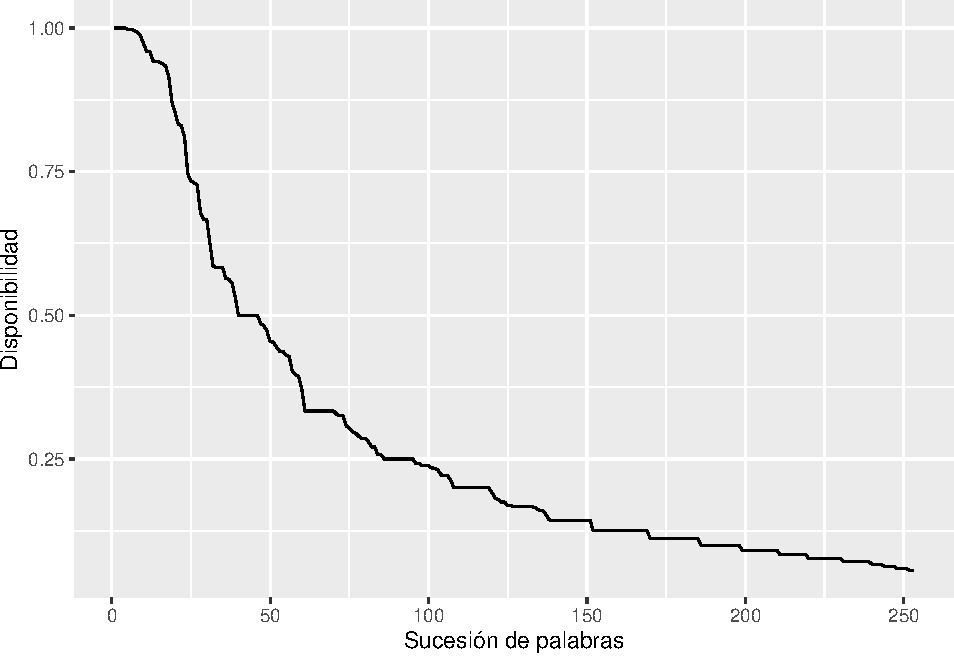
\includegraphics[width=6.50in,height=30.25in,keepaspectratio]{PresentacionCentralex_files/figure-latex/unnamed-chunk-29-1.png}

Mediante un diagrama de puntos, en el que se representan en cada eje las
disponibilidades para hombres y mujeres, pero sólo de aquellos términos
que no se han clasificado en el mismo nivel, y etiquetando por
diferencia de nivel, se obtendría:

\begin{Shaded}
\begin{Highlighting}[]
\NormalTok{levelsSexo <-}
\StringTok{  }\KeywordTok{inner_join}\NormalTok{(levelsHombres }\OperatorTok
\StringTok{               }\KeywordTok{select}\NormalTok{(centers,level,words,availability) }\OperatorTok
\StringTok{               }\KeywordTok{rename}\NormalTok{(}\DataTypeTok{avHombre=}\NormalTok{availability,}\DataTypeTok{levelHombre=}\NormalTok{level),}
\NormalTok{             levelsMujeres }\OperatorTok\StringTok{  }
\StringTok{               }\KeywordTok{select}\NormalTok{(centers,level,words,availability) }\OperatorTok
\StringTok{               }\KeywordTok{rename}\NormalTok{(}\DataTypeTok{avMujer=}\NormalTok{availability,}\DataTypeTok{levelMujer=}\NormalTok{level), }
           \DataTypeTok{by=}\KeywordTok{c}\NormalTok{(}\StringTok{"centers"}\NormalTok{,}\StringTok{"words"}\NormalTok{)) }
\NormalTok{levelsSexo }\OperatorTok
\StringTok{  }\KeywordTok{filter}\NormalTok{(levelHombre }\OperatorTok{!=}\StringTok{ }\NormalTok{levelMujer) }\OperatorTok
\StringTok{  }\KeywordTok{mutate}\NormalTok{(}\DataTypeTok{diffLevel=}\KeywordTok{factor}\NormalTok{(}\KeywordTok{abs}\NormalTok{(levelHombre}\OperatorTok{-}\NormalTok{levelMujer))) }\OperatorTok
\StringTok{  }\KeywordTok{ggplot}\NormalTok{(}\KeywordTok{aes}\NormalTok{(}\DataTypeTok{x=}\NormalTok{avHombre,}\DataTypeTok{y=}\NormalTok{avMujer,}\DataTypeTok{color=}\NormalTok{diffLevel)) }\OperatorTok{+}\StringTok{ }\KeywordTok{geom_point}\NormalTok{() }\OperatorTok{+}
\StringTok{  }\KeywordTok{theme_bw}\NormalTok{() }\OperatorTok{+}\StringTok{ }\KeywordTok{scale_colour_grey}\NormalTok{()}
\end{Highlighting}
\end{Shaded}

\includegraphics{PresentacionCentralex_files/figure-latex/unnamed-chunk-30-1.pdf}

Se puede observar que en la mayor parte de los casos en los que se
clasifican en niveles distintos, lo hacen con poca diferencia.

\begin{Shaded}
\begin{Highlighting}[]
\NormalTok{diffs <-}\StringTok{ }\KeywordTok{tapply}\NormalTok{(levelsSexo}\OperatorTok{$}\NormalTok{levelHombre }\OperatorTok{==}\StringTok{ }\NormalTok{levelsSexo}\OperatorTok{$}\NormalTok{levelMujer, }
\NormalTok{                levelsSexo}\OperatorTok{$}\NormalTok{centers, }
\NormalTok{                mean) }\OperatorTok{*}\StringTok{ }\DecValTok{100} 
\NormalTok{diffs}
\end{Highlighting}
\end{Shaded}

\begin{verbatim}
##       01       02       03       04       05       06       07       08 
## 71.66667 57.31707 60.00000 66.27907 66.20690 61.64384 71.42857 64.83516 
##       09       10       11       12       13       14       15       16 
## 66.66667 65.57377 71.42857 74.68354 65.15152 69.11765 64.95726 73.68421 
##       17       18       19       20 
## 71.30435 66.00000 73.77049 67.17557
\end{verbatim}

\begin{Shaded}
\begin{Highlighting}[]
\KeywordTok{summary}\NormalTok{(diffs)}
\end{Highlighting}
\end{Shaded}

\begin{verbatim}
##    Min. 1st Qu.  Median    Mean 3rd Qu.    Max. 
##   57.32   65.10   66.47   67.44   71.43   74.68
\end{verbatim}

De hecho, se puede observar que el porcentaje de términos clasificados
en el mismo nivel en cada centro de interés va entre el 57 y el 74 por
ciento.

\end{document}
